\documentclass[9pt,twocolumn,twoside]{styles/osajnl}
\usepackage{fancyvrb}
\usepackage[colorinlistoftodos,prependcaption,textsize=normal]{todonotes}
\newcommand{\TODO}[2][]{\todo[color=red!10,inline,#1]{#2}}
\newcommand{\GE}{\TODO{Grammar}}
\newcommand{\SE}{\TODO{Spelling}}
\newcommand{\TE}{\TODO{Term}}
\newcommand{\CE}{\TODO{Citation}}
\journal{i524} 

\title{\LaTeX\ Linux Containers - Virtualization for  Cloud Era}

\author[1]{Ashok Vuppada}

\affil[1]{School of Informatics and Computing, Bloomington, IN 47408, U.S.A.}

\affil[*]{Corresponding authors: ashokmadhu66@gmail.com}

\dates{paper-1, \today}

\ociscodes{LXC,Cloud, I524}

% replace this with your url in GitHub/gitlab
\doi{\url{https://github.com/justbbusy/sp17-i524/tree/master/paper1/S17-IO-3024/report.pdf}}


\begin{abstract}
In todays world , cloud is seen as delivery model for growing number
of enterprises as the benefits of agility and efficiencies are better
understood and available. The concept of virtualization is one of the
building blocks for cloud infrastructure and services offering.The
traditional VM work with hardware emulation causing inefficient
resource and storage management. New technology ‘Linux containers’
build with the concept of ‘Operating system Virtualization’ aims at
efficient resource management and customization. 
\end{abstract}

\setboolean{displaycopyright}{true}

\begin{document}

\maketitle

\TODO{This review document is provided for you to achieve your
  best. We have listed a number of obvious opportunities for
  improvement. When improving it, please keep this copy untouched and
  instead focus on improving report.tex. The review does not include
  all possible improvement suggestions and if you sea comment you may
  want to check if this comment applies elsewhere in the document.}
\TODO{some punctuation used in Abstract are not English}

\section{Introduction}

Traditional Hyperviser based Virtualization works with the idea of
creating virtual hardware and running guest operating system on
them. Applications are then expected to run on the guest operating
system. The hypervisor layer would control the different guest
operating systems.This model offers great deal of isolation,however
the disadvantage of the this set up is each of the guest operating
system would let a kernel process ( memory and cpu manager processes)
run on the host operating system and causing the performance overhead
and resource constrain. It is also noted that each of the guest
operating system runs from the ISO file ( usually in GBs) causing
limitations on the storage of the host. \cite{www-slashroot} 

Container based virtualization works with the similar concept except
eliminating the need of hypervisor layer. Each instance of the guest
operating system can be assumed as any other processes running on the
host system. There would be only one kernel processing running on the
host operating system ( that belong to the host OS ) and it would
shared with the guest operating systems. The hardware resources ( CPU
and memory ) will also be shared. Since there is single process
controlling the memory and CPU usage is running this model has
performance advantage \cite{www-slashroot}

\begin{figure}[htbp]
\centering
\fbox{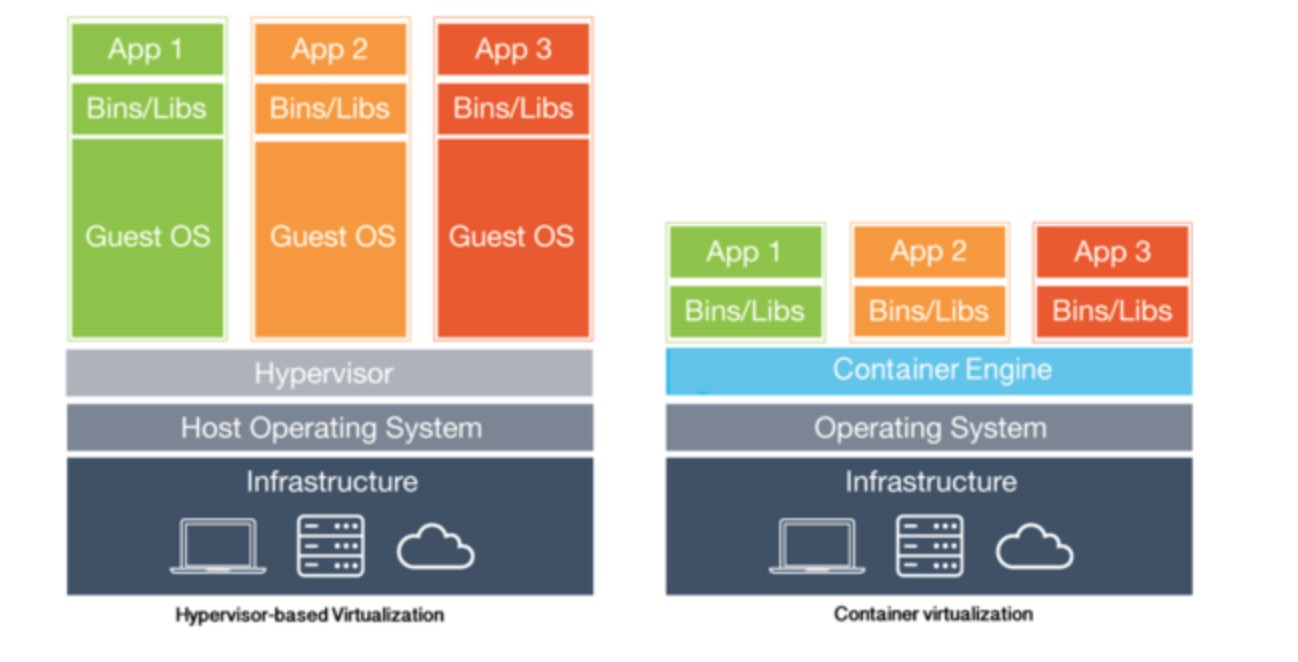
\includegraphics[width=\linewidth]{images/VM.jpg}}
\caption{Architecture Comparison of Hypervisor Based VM and containers.}
\label{fig:false-color}
\end{figure}
\TODO{you have nice figures. first, please cite them if it is not made by yourself. also, you need to
mention these figures "as shown in fig X..."}

\section{Building Blocks}

 Linux containers are built on the modern kernel features like
‘chroots’ , ‘namespaces’ ,’cgroups’ and Linux security models and
mandatory access controls.\cite{www-bondner}
\begin{itemize}
\item chroot :
its a way of isolating a process to change only defined file
system.The process running inside the chroot jail cannot act on the
file system out side it. this is used to isolate the unstable
applications to hamper the file system in use.\cite{www-ubuntu}
\item namespaces:
namespaces provides the process level isolation for the global
resources.It helps the process in each of the namespace to believe its
the only process.\cite{www-bondner}
\item cgroups: 
its a kernel feature which allows to
allocate resources to a given group of process(s).it helps one
allocating and accounting CPU time, memory etc for a set of
processes\cite{www-infoworld}
\item  Linux Security module:
 “Linux Security Modules (LSM) is a
framework that allows the Linux kernel to support a variety of
computer security models while avoiding favoritism toward any single
security implementation”.\cite{www-wiki-LSM}
\item Mandatory Access control: 
Its is process\TE
by which the security policies setup cannot gets overrides by a
user. \cite{www-linux}
\end{itemize} 
Linux containers are built on kernel features stated , as they are linux
features the contender concept is not available in Microsoft windows. 

\section{Project LXC AND DOCKER}
Both LXC and Docker are the practical implementations of the linux
containers.  LXC is the original linux container developed.The project
docker was initially started with the idea of extending LXC but ended
up developing its own container. The key difference between LXC and a
docker is in LXC each virtual container would allow multiple process
to run where as in docker each process would need a separate docker
container.Docker is designed to be stateless and credited for its
portability. Because of the overwhelming popularity of docker it is
often treated as synonym for linux containers .The below diagram
depicts the main structural differences between LXC and docker.\cite{www-lxc-docker}

\begin{figure}[htbp]
\centering
\fbox{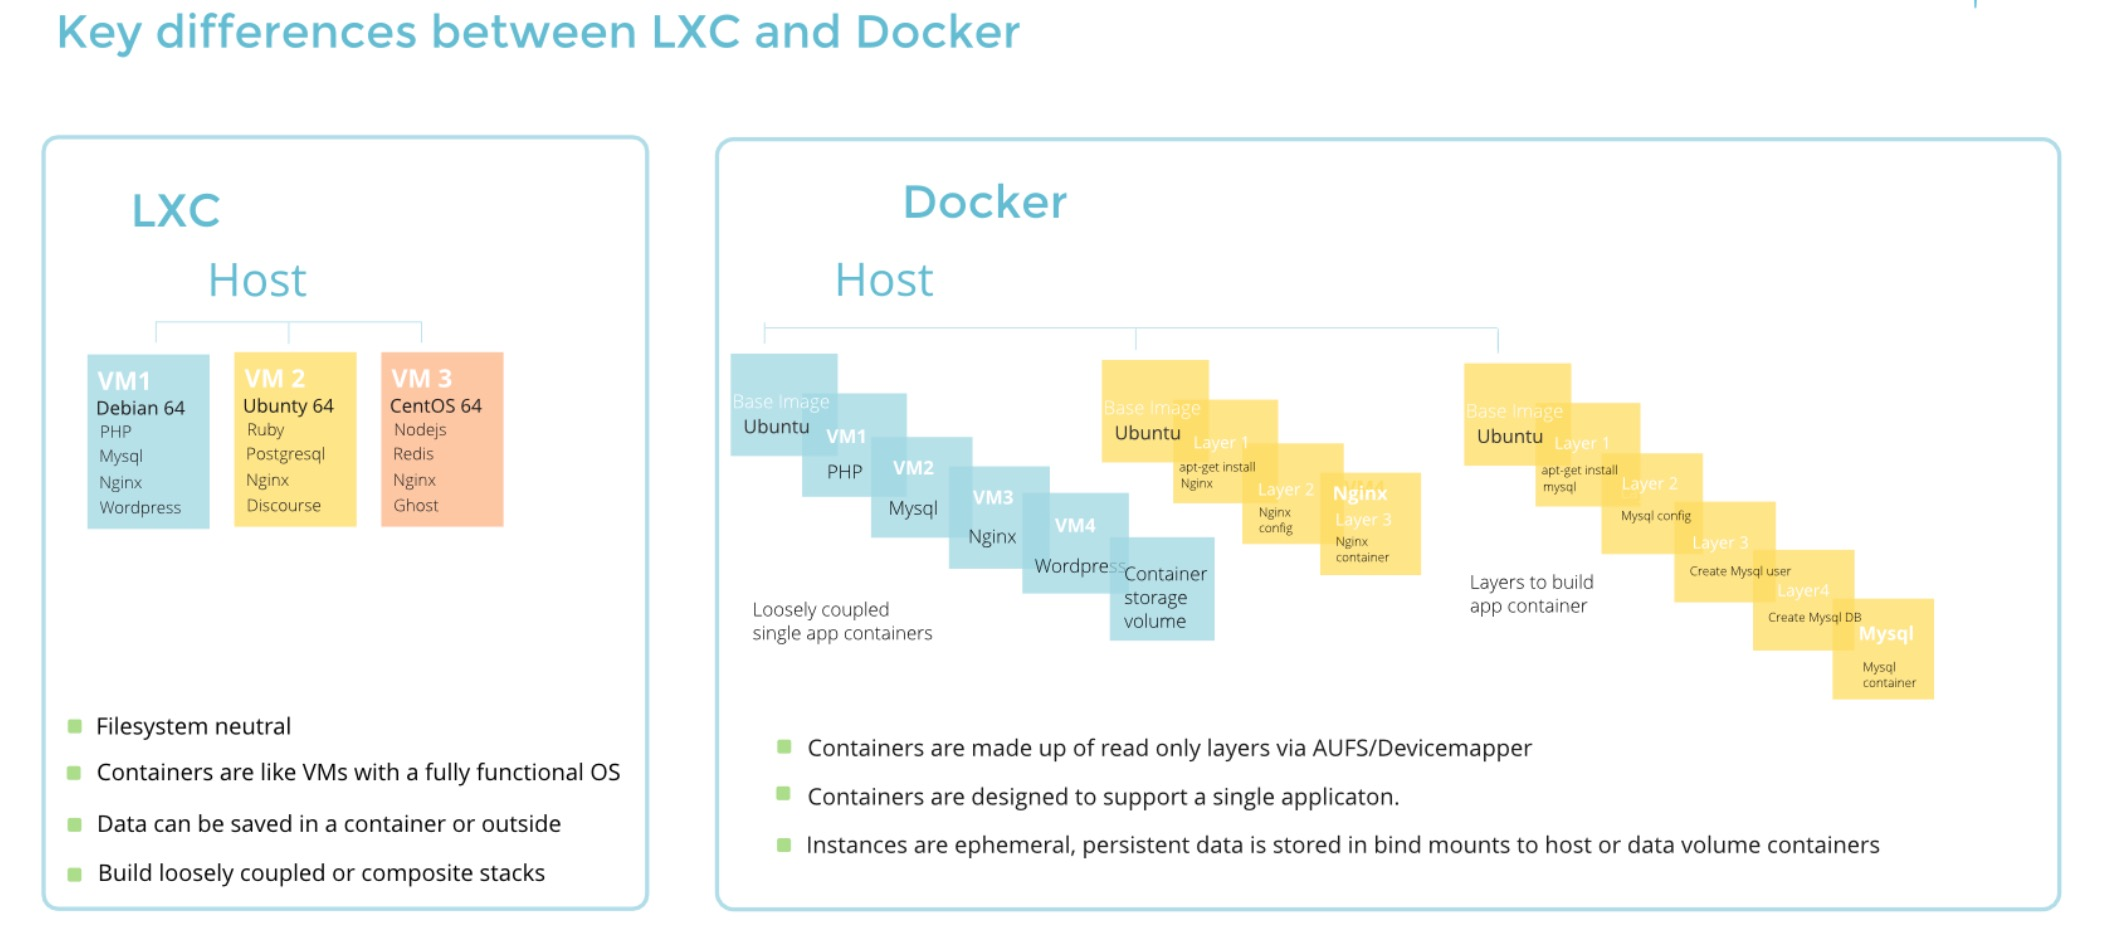
\includegraphics[width=\linewidth]{images/Docker.jpg}}
\caption{Architecture Comparison of LXC and Docker.}
\label{fig:false-color}
\end{figure}
\section{performance Comparison} \cite{www-semantics}
In this study , Linux on KVM is studied for Hypervisor based VM , LXC
and docker are compared as container based solutions. OSv is used as
light weight guest OS.
\TODO{let's not start a sentense with a citation}

\begin{enumerate}

\begin{figure}[htbp]
\centering
\fbox{\includegraphics[width=\linewidth]{images/Score.jpg}}
\caption{Single Core Perf Comparison}
\label{fig:false-color}
\end{figure} 

\item CPU Performance \\  
CPU multithreaded performance is measured with a benchmark called 'Y
Cruncher' which calculate the values of Pi the results can be seen
from the table below 
  NBENCH is used for single core comparison producing three different
  indexes: Integer Index, Floating Point Index, and Memory
  Index. Please see the blow diagram from the comparison
\begin{figure}[htbp]
\centering
\fbox{\includegraphics[width=\linewidth]{images/Mcore.jpg}}
\caption{Multi Core Perf Comparison}
\label{fig:false-color}
\end{figure} 





\item Memory Performance \\
 Below are test results  using STREAM 
\begin{figure}[htbp]
\centering
\fbox{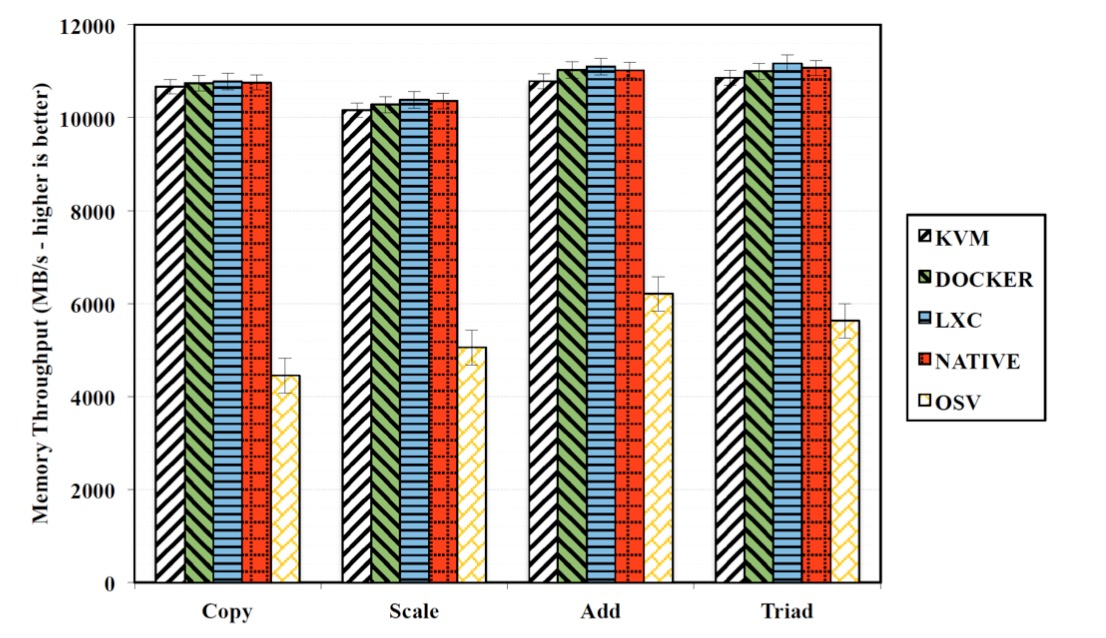
\includegraphics[width=\linewidth]{images/Memory.jpg}}
\caption{Memory Perf Comparison}
\label{fig:false-color}
\end{figure}

\item Disk I/O Performance \\
   Bonnie++ is used to measure the disk performance and below are the
   results.
\begin{figure}[htbp]
\centering
\fbox{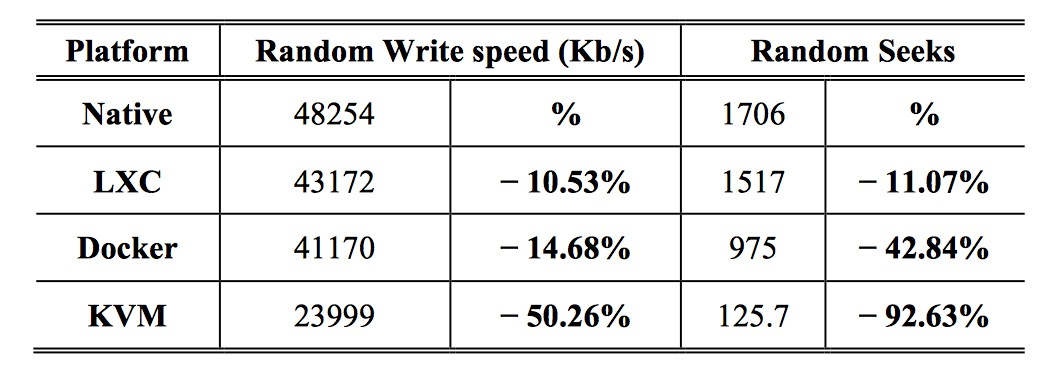
\includegraphics[width=\linewidth]{images/DiskIO.jpg}}
\caption{Disk IO Perf Comparison}
\label{fig:false-color}
\end{figure}

\item Network I/O Performance \\
Network  I/O is measured with Netperf \\
\begin{figure}[htbp]
\centering
\fbox{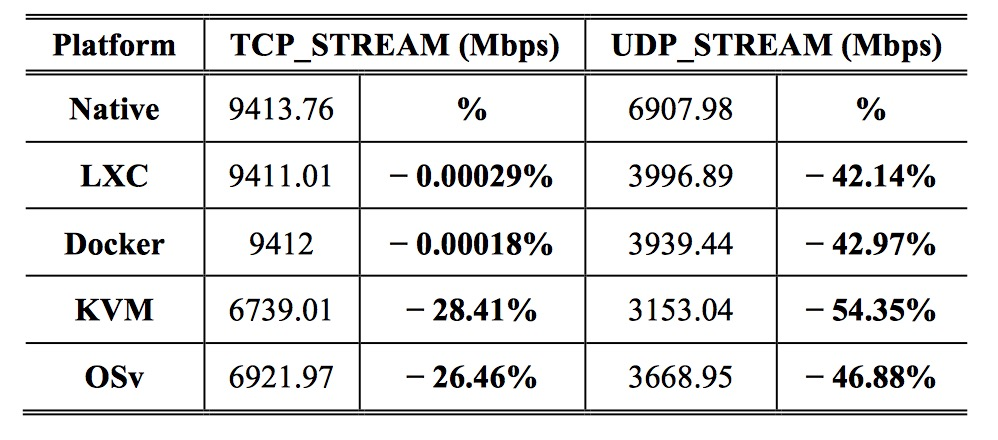
\includegraphics[width=\linewidth]{images/NetworkIO.jpg}}
\caption{Network IO Comparison}
\label{fig:false-color}
\end{figure}


\end{enumerate}

This test concludes that containers performed well but needs to
improve on security and isolation. 

\section{Use Cases}\cite{www-virtual}
\TODO{why you have a citation right after the section title?}
\begin{enumerate}
\item Continous Integration \\
With the concept of DevOps there is a tight integration between the
development and Operations.The frequency of deploying new
applications had increased tremondously.With multiple applications to
be deployed with along with the dependencies,Op team used to have
tough time, Container with the portability and packaging made the job
easy. \cite{www-virtual}
\item Container as a service \\
This concept is similar to the PaaS, In a complex IT structure of an
organization it was difficult to manage different existing
technologies and add a new one,but with container as a service the new
technology container image can be built and hosted on the existing
host for the development to happen. This model eliminates the need of
learning the dependencies associated with running multiple applications
on the same host. \cite{www-virtual}
\item Micro Services \\
The idea of Micro service is to have the isolation between the
application processes as much as possible so the each of the
application can be built in the best technology
suitable. This model is very helpful for modernization of the
applications easily. Since container installation takes few seconds
and doesn't come with the lot of dependencies they are the best choice
for Microservices. \cite{www-virtual}
\end{enumerate}

\section{LIMITATIONS} \cite{www-search}

\begin{enumerate}
\item Containers are not suitable for all the purposes , some of the
  existing applications are designed best for sharing the physical
  layer of the machine.If scalability and fast deployment are not
  really applicable there is no good reason to use containers. \cite{www-search}  
\item Containers provides weaker isolation compare the hypervisor
  based virtual machines.Since they share the common kernel process,
  if there is some bug or virus on the host there would be chance to
  propgate to other containers. \cite{www-search}
\item Containers are presently getting evolved,compared to the
  existing traditional VMs the tools available for monitoring the
  resources on containers are limited. \cite{www-search}

\item containers are build on the kernel features build in Linux,Hence
  this cannot be directly used by other operating systems which does't
  have Linux kernel ( Microsoft Windows) 
\end{enumerate}

\section{Conclusion} 
In the era of cloud computing and micro services the need and
popularity of containers are gradually growing up.Docker with its
ability of “Build Ship Run” \cite{www-docker} ability made the container concept
more popular and useful.But eventually its not going to replace the
traditional hypervisor based virtual machines any time soon ( as they
are far more superior interns of security and integration compared to
containers). Both the technologies needs to be used in conjunction to
get the better of both the worlds. 


\bibliography{references}
 
\newpage

\appendix
\end{document}
